%doc
\documentclass[a4paper,graphics,14pt]{article}
\pagenumbering{arabic}
\usepackage[margin=1in]{geometry}

%packages
\usepackage[utf8]{inputenc}
\usepackage{amsfonts}
\usepackage[T1]{fontenc}
\usepackage{lmodern}
\usepackage[ngerman]{babel}
\usepackage{booktabs}
\usepackage{amsmath}
\usepackage{amssymb}
\usepackage{mathtools}
\usepackage{setspace}
\usepackage{setspace}
\usepackage{listings}
\usepackage{color}
%\usepackage[left=3cm,right=3cm,top=1cm,bottom=4cm]{geometry}


%Code integrieren
\definecolor{gray}{rgb}{0.96,0.96,0.96}
\lstset{
	language=java,
	basicstyle=\ttfamily,
	numbersep=5pt,
	backgroundcolor=\color{gray},
	showspaces=false,
	frame=single,
	tabsize=2,
	breaklines=true,
	prebreak={\textbackslash}
}
\lstset{literate=%
  {Ö}{{\"O}}1
  {Ä}{{\"A}}1
  {Ü}{{\"U}}1
  {ß}{{\ss}}1
  {ü}{{\"u}}1
  {ä}{{\"a}}1
  {ö}{{\"o}}1
}


\author		{ \Large Danje Petersen, 379748}
\title{ \Huge Datenstrukturen \& Algorithmen \\
		\huge Übungsblatt 07 | Tutorium 2}
\date{27.05.2019}


%commands
\newcommand{\aufgabe}[1]{\section*{Aufgabe #1}}
\newcommand{\apt}[1]{\subsection*{#1} }
\newcommand{\RM}[1]{\MakeUppercase{\romannumeral #1{}}}


\begin{document}

\doublespacing
\maketitle
\onehalfspacing

\aufgabe{H19}

\apt{a)}

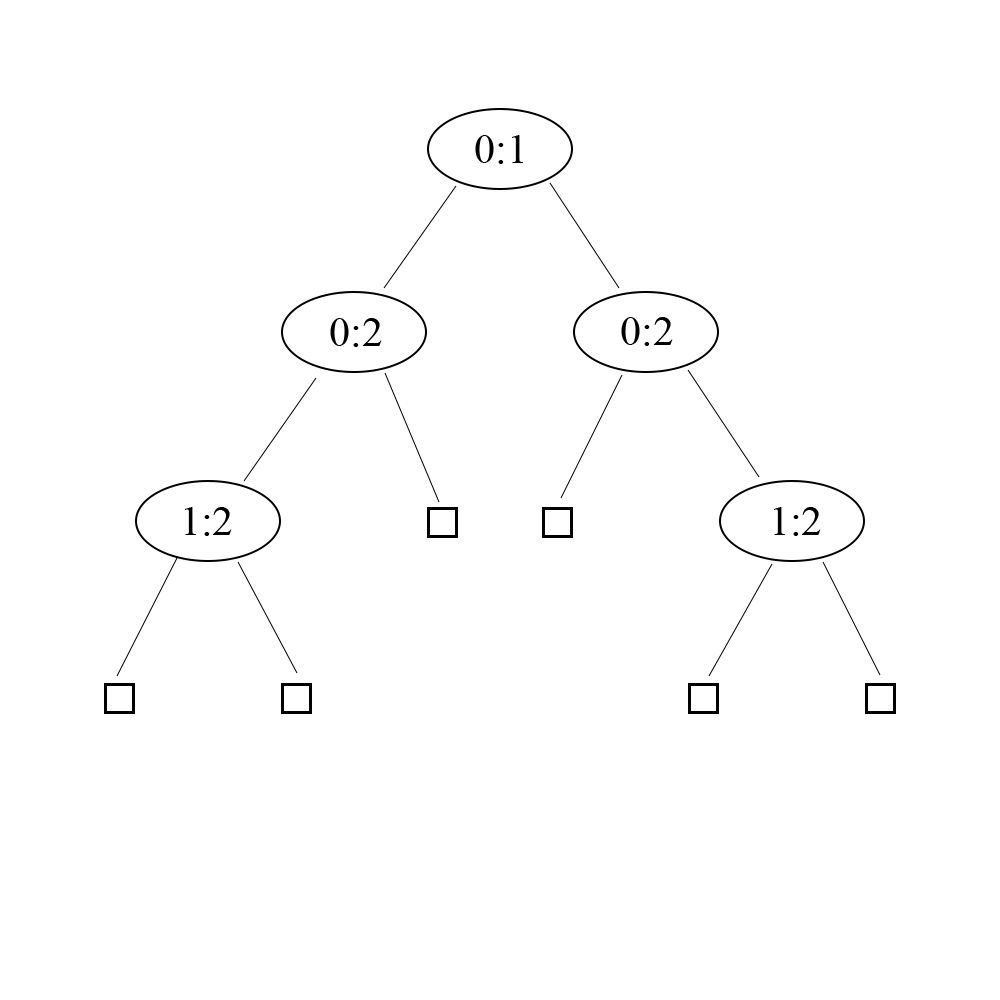
\includegraphics[scale=0.3]{Vergleichsbaum.png}

Es ist möglich die Richtige Reihenfolge zu finden.



\apt{b)}
Von den 6 Permutationen benötigen 4 drei Vergleiche und 2 zwei Vergleiche (siehe Vergleichsbaum in a)).
\begin{center}
\[ 3 * \frac{2}{3} + 2 * \frac{1}{3} \] \\ 
\[ = \frac{6}{3} + \frac{2}{3} = \frac{8}{3} = 2,66 \]
\end{center}


\aufgabe{H20}

\apt{a)}
Bei n = 6 werden bei dem Array [3,1,2,6,5,4] maximal 2 Einträge auf dem Stack gespeichert.
Dies entspricht $\frac{1}{3} * n$ und fällt somit unter $\Omega(n)$.

\apt{b)}
Der Speicherverbrauch lässt sich auf $O(\log{(n)})$ indem man bei jeder Auswahl des Pivot Elements ein Minimum sucht und dieses wählt. Somit steht immer nur ein Eintrag im Stack also $\frac{1}{n} \subset O(\log{(n)}$. Allerdings würde dies die Laufzeit stark beeinträchtigen. 

\apt{c)}
Ja, die Permutationen der verbleibenden Elemente sind gleich wahrscheinlich, weil kein Element aufgrund seines Wertes seine Position verändert, sondern zufällig.



\aufgabe{H21}

\begin{figure}[h]
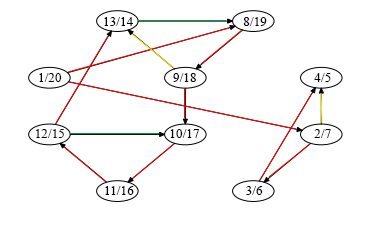
\includegraphics[width=0.8\textwidth]{Tiefensuche.png}
\caption{rot = Baumkante, gelb = Vorwärtskante, grün = Rüchwärtskante}
\end{figure}



\end{document}